\section{Methodology}
\label{sec:method}

Developing generalizable foundation models for EEG is hindered by two primary obstacles: the \textbf{topological heterogeneity} of EEG montages (varying channel counts and layouts) and the \textbf{computational complexity} of attention mechanisms. Standard models struggle with diverse input channel configurations, limiting data aggregation and generalizability. Furthermore, transformer-based approaches often face prohibitive \(\bigO((C \cdot S)^2)\) or \(\bigO(\max(C^2, S^2))\), as discussed in the section \ref{subsec:related_work}, complexity when processing \(C\) channels and \(S\) temporal patches. This limits their applicability to high-density EEG or long recordings.

LUNA addresses these challenges using a smaller latent space. Firstly, Channel-Unification Module (Sec .~\ref {subsubsec:channel_unification}) employs learned queries and cross-attention to project variable-channel features into a fixed-dimension latent space, achieving topology invariance. Secondly, by unifying channel information into a compact set of \(Q\) queries (\(Q \ll C\)) before temporal processing, LUNA significantly reduces computational demands. This design enables efficient and scalable processing of heterogeneous EEG data, paving the way for more robust foundation models. LUNA adopts an encoder-decoder architecture that transforms EEG signals from heterogeneous montages into a unified latent representation, enabling topology-agnostic modeling and efficient downstream decoding (Figure~\ref{fig:methodlogy}).

\begin{figure}[htpb!]
    \centering
    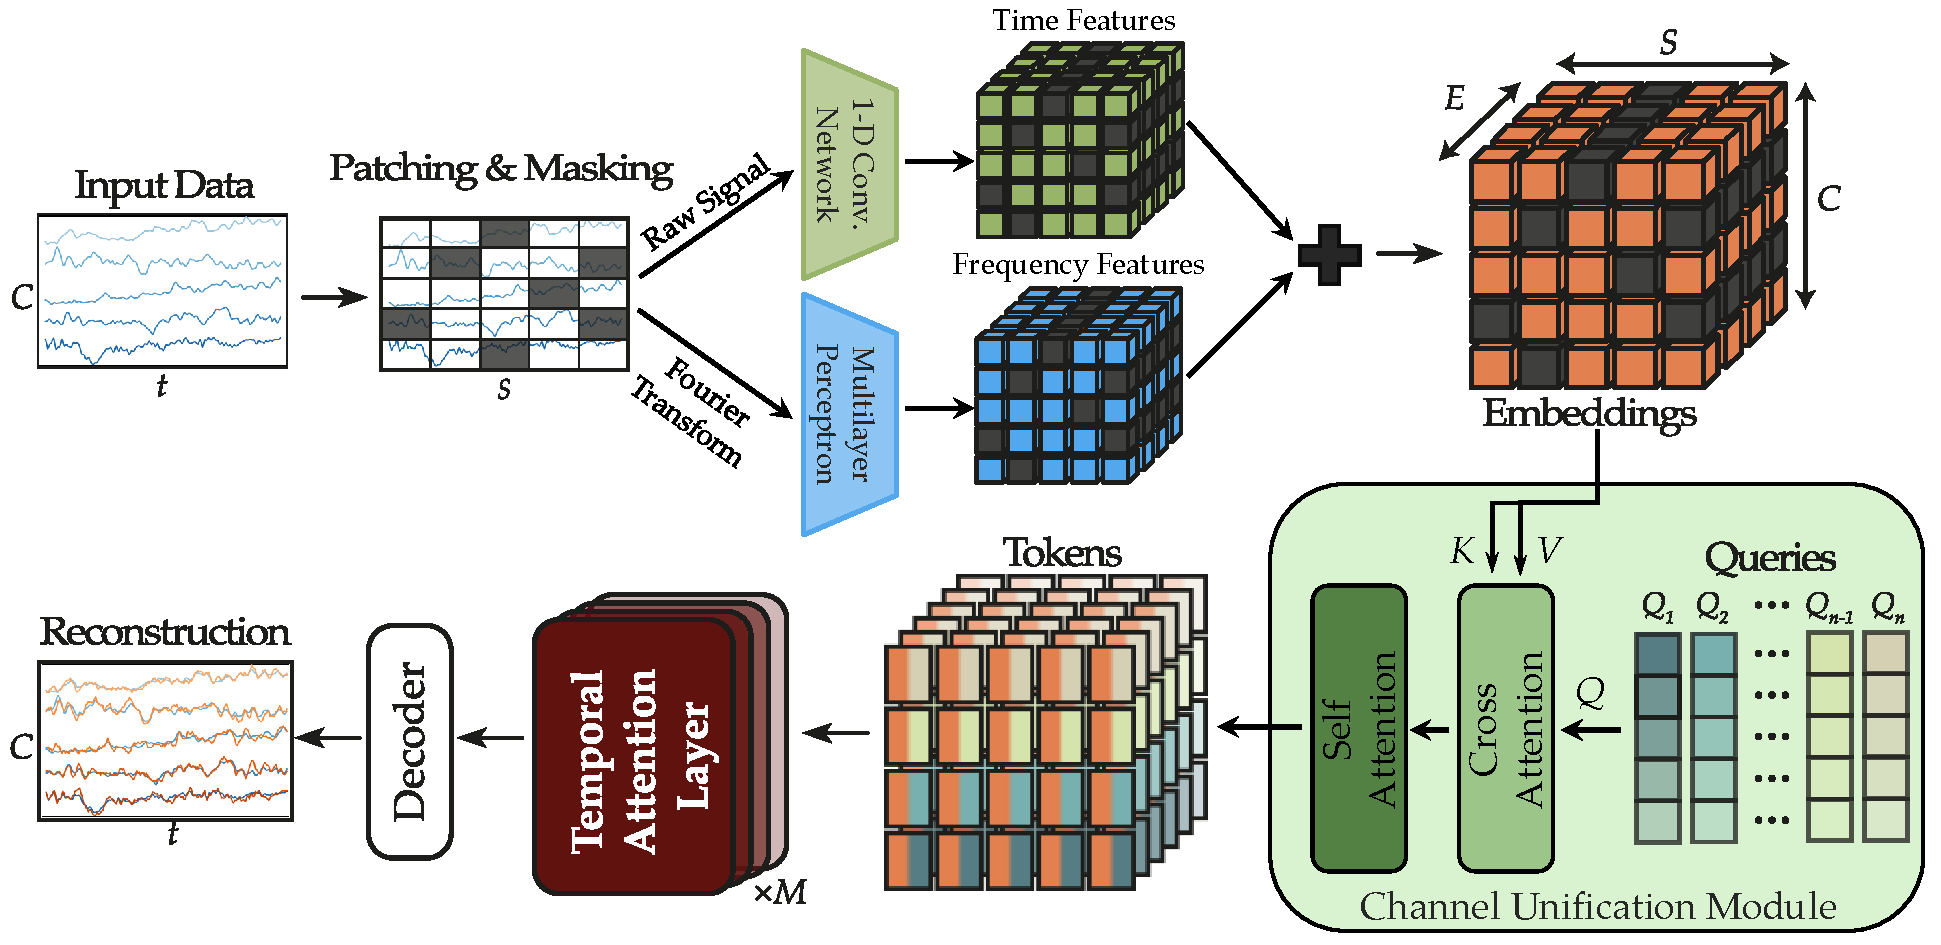
\includegraphics[width=\linewidth]{figs/methodology_2.pdf}
    \caption{Overview of LUNA. EEG signals ($B \times C \times T$) are segmented into patches and embedded. Channel-Unification Module maps channel-wise features into a fixed-size latent space using learned queries ($Q$). Patch-wise Temporal Attention processes this latent sequence. The decoder generates task-specific outputs.}
    \label{fig:methodlogy}
\end{figure}

\subsection{Encoder}
The encoder comprises three key modules that transform the input EEG into a topology-agnostic latent representation: patch feature extraction, channel unification, and patch-wise temporal modeling.

\paragraph{Patch Feature Extraction}
Given raw EEG \(x \in \mathbb{R}^{B \times C \times T}\) (Batch \(B\), Channels \(C\), Time \(T\)), we segment each channel into \(S = T / P\) non-overlapping temporal patches of size \(P\). These patches are embedded via two parallel pathways:

\textbf{Temporal Embedding:} A 1D convolutional network (with GroupNorm~\citep{wu2018group}, GELU~\citep{hendrycks2016gaussian}) encodes local temporal features similar to state-of-the-art methods such as LaBraM\cite{jiang2024large} and CBraMod \cite{wang2024cbramod},
\textbf{Frequency Embedding:} The magnitude and phase from each patch's Fourier transform are projected through an MLP.
These representations are summed to obtain patch features \(x_\text{features}\).

\vspace{-3mm}
\paragraph{Channel Positional Encoding}
To encode electrode locations, we apply NeRF-inspired sinusoidal encoding~\cite{mildenhallNerf} to normalized 3D electrode coordinates, followed by an MLP projection. This yields $\mathbf{E}_{\text{pos}} \in \mathbb{R}^{B \times C \times E}$, which is added to $x_{\text{features}}$. 

During pre-training, a random subset of tokens is masked using a learnable embedding. 

\paragraph{Channel-Unification Module}
\label{subsubsec:channel_unification}
To handle varying channel counts (\(C\)) across recordings, we introduce a cross-attention module that maps patch-wise features into a fixed latent space. Specifically, Q learned queries $\mathbf{Q}_{\text{learn}} \in \mathbb{R}^{Q \times E}$, (learnable parameters \emph{without} a batch dimension, initialized orthogonally) cross-attend to patch features. For attention, these queries are repeated across the $B \cdot S$ patch instances as $\tilde{\mathbf{Q}} \in \mathbb{R}^{(B \cdot S) \times Q \times E}$.

Let the input to this module be the tensor \( \mathbf{X}_\text{token} \in \mathbb{R}^{B \times (C \cdot S) \times E} \), representing the spatially-aware features for \(B\) samples, \(S\) patches per channel, and feature dimension \(E\). We first reshape this tensor to \( \mathbf{X}' \in \mathbb{R}^{(B \cdot S) \times C \times E} \) to treat each patch instance across the batch independently while isolating the channel dimension for attention.

The cross-attention mechanism then computes the output representation \( \mathbf{A}_{\text{out}} \in \mathbb{R}^{(B \cdot S) \times Q \times E} \):
\begin{equation}
    \mathbf{A}_{\text{out}} = \text{MultiHeadAttention}(\tilde{\mathbf{Q}}, \mathbf{X}', \mathbf{X}')
\end{equation}


A feed-forward network (FFN) with residual connection refines the outputs, followed by $L$ Transformer encoder layers operating on the query dimension $Q$.
\begin{equation}
    \mathbf{X}_{\text{unified}} = \text{TransformerEncoder}(\mathbf{A}_{\text{out}} + \text{FFN}(\mathbf{A}_{\text{out}}))
\end{equation}
The result \( \mathbf{X}_{\text{unified}} \in \mathbb{R}^{(B \cdot S) \times Q \times E} \) decouples further processing from the original electrode layout.  \textit{For clarity: learnable tensors (e.g., $\mathbf{Q}_{\text{learn}}$) omit the batch dimension; repetition occurs only at attention time (e.g., $\tilde{\mathbf{Q}}$).} 

\paragraph{Patch-wise Temporal Encoder}
\label{subsubsec:temporal_encoder}

The unified representations are reshaped into temporal sequences \( \mathbf{X}_{\text{unified}}' \in \mathbb{R}^{B \times S \times (Q \cdot E)} \). These are processed by a stack of Transformer encoder blocks with Rotary Positional Embeddings (RoPE)~\citep{su2024roformer} to capture temporal dependencies efficiently. A key advantage of this encoding approach is that each of the \(S\) temporal tokens in \(\mathbf{X}_{\text{unified}}'\) now encapsulates richer, aggregated information from multiple input channels, rather than representing a single channel's segment. Furthermore, by not tokenizing each channel independently for temporal processing, the effective sequence length for the temporal Transformers is reduced from \(S \cdot C\) to just \(S\), leading to significant reductions in computational complexity and memory requirements. $$E_{\text{out}} = \text{TemporalEncoder}(\mathbf{X}_{\text{unified}}')$$

\subsection{Decoder}
\label{subsec:decoder}
LUNA supports two decoding strategies depending on the task: reconstruction (pre-training) and classification (fine-tuning).


\paragraph{Reconstruction Head (Pre-training)}
For masked patch reconstruction, $C$ learned decoder queries $\mathbf{E}_{\text{dec}}^{\text{learn}} \in \mathbb{R}^{C \times E}$ (learnable parameters \emph{without} a batch dimension) are repeated across the batch and patches as $\tilde{\mathbf{E}}_{\text{dec}} \in \mathbb{R}^{(B \cdot S) \times C \times E}$ and attend to reshaped $E_{\text{out}}$ via cross-attention, producing channel-specific representations $\mathbf{Z}_{\text{dec}} \in \mathbb{R}^{(B\cdot S) \times C \times E}$. $E_{\text{out}} \in \mathbb{R}^{B \times S \times (Q \cdot E)}$ is reshaped to be used as keys/values $\mathbf{K}, \mathbf{V} \in \mathbb{R}^{(B \cdot S) \times Q \times E}$ for attention. A linear projection $\phi:\mathbb{R}^{E}\!\rightarrow\!\mathbb{R}^{P}$ applied on $\mathbf{Z}_{\text{dec}}$  recovers the patch values. 
{\textit{Decoder queries are indexed by channel labels and can be reused across datasets when electrodes overlap; this reconstruction head is used only during pre-training.}



\paragraph{Classification Head (Fine-tuning)}
For downstream tasks, a single aggregation query $\mathbf{E}_{\text{agg}}^{\text{learn}} \in \mathbb{R}^{1 \times (Q \cdot E)}$ (no batch) is repeated across the batch as $\tilde{\mathbf{E}}_{\text{agg}} \in \mathbb{R}^{B \times 1 \times (Q \cdot E)}$ and attends to $E_{\text{out}}$ to produce a pooled representation, which is passed to an MLP for classification.


\subsection{Training Objectives}
\label{subsec:training}
LUNA is pre-trained with a masked reconstruction loss and an auxiliary query specialization loss.

\paragraph{Reconstruction Loss}
A Smooth L1 loss is applied to both masked and visible patches:
$$L_{rec}=\frac{1}{N_\text{masked}} \sum_{i \in M} \text{SmoothL1}(x_{\text{orig}_i}, x_{\text{recons}_i})+\alpha \cdot \frac{1}{N_\text{visible}} \sum_{i \notin M} \text{SmoothL1}(x_{\text{orig}_i}, x_{\text{recons}_i})$$

and SmoothL1($x, \hat{x}$) = $0.5(x - \hat{x})^2$ if $|x - \hat{x}| < \beta$, else $\beta|x - \hat{x}| - 0.5\beta^2$, with $\beta=1$.
\paragraph{Affinity matrix.}
Let $\mathbf{A}_{\text{attn}} \in \mathbb{R}^{B' \times H \times Q \times C}$ denote the cross-attention weights (queries $\rightarrow$ channels) from the channel-unification module, for $B'$ instances and $H$ heads. We define
\[
\mathbf{A}_{\text{affinity}} \;=\; \frac{1}{H}\sum_{h=1}^{H} \mathbf{A}_{\text{attn}}[:,h,:,:] \;\in\; \mathbb{R}^{B' \times Q \times C},
\]
i.e., attention weights averaged over heads, so that $(\mathbf{A}_{\text{affinity}})_{b',q,c}$ measures the affinity between query $q$ and channel $c$ for instance $b'$.
\paragraph{Query Specialization Loss}
To promote diversity among queries, we penalize similarity in query-channel affinity matrices by minimizing the mean value of off-diagonal elements:
\begin{equation*}
    \mathcal{L}_{\text{spec}} = \frac{\lambda_{\text{spec}}}{B' \cdot Q \cdot (Q-1)} \sum_{b'=1}^{B'} \sum_{i=1}^{Q} \sum_{j=1, j \neq i}^{Q} \left( (\mathbf{A}_{\text{affinity}} \mathbf{A}_{\text{affinity}}^T)_{b', i, j} \right)^2
\end{equation*}